\documentclass[12pt,a5paper]{article}
\usepackage{amsmath,defns,reducecode,natbib}
\IfFileExists{ajr.sty}{\usepackage{ajr}}{}
\Cal L

\usepackage{pgfplots}

\usepackage{pdfcomment}
\newcommand{\ajr}[1]{%
  \pdfcomment[author=AJR,color={1 1 0},subject={#1}]{#1}}
%\AtBeginDocument{\listofpdfcomments}
\atBegin{tableofcontents}{\listofpdfcomments}

\title{Discretisation of nonlinear Schrodinger PDE with periodic potential---modified for coupling via averages over cores and action regions}
\author{AJR}
\date{\today}

\begin{document}

\maketitle

\tableofcontents

\section{Introduction}

The immediate aim is to model the dynamics in just one space dimension of the nonlinear Schrodinger \pde~\eqref{eq:nls} with periodic potential.
That is, we seek to model the field~\(u(x,t)\) that solves 
\begin{equation}
-i\D tu=\DD xu-V(x)u-\sigma |u^2|u
%\quad\text{and}\quad
%+i\D tv=\DD xv-V(x)v-\sigma uv^2
\label{eq:nls}
\end{equation}
where here, for example and as illustrated by Figure~\ref{fig:twopotl}, we could take potential 
\begin{figure}
\centering
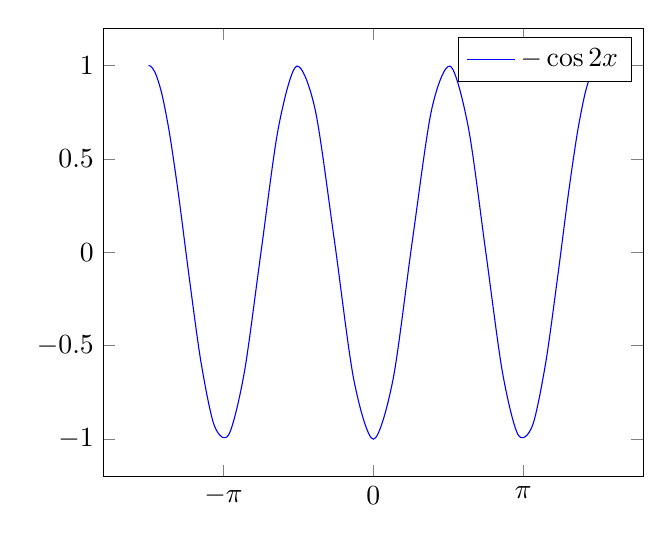
\begin{tikzpicture} 
\begin{axis}[ domain=-90:90 ,samples=37
    ,xtick={-3.14,0,3.14},xticklabels={$-\pi$,$0$,$\pi$}]
\addplot+[smooth,no marks]({3*pi/2*sin(x)},{-cos(deg(2*3*pi/2*sin(x)))});
\addlegendentry{$-\cos 2x$}
\end{axis}
\end{tikzpicture}
\caption{Wannier potential \(V(x)=A\cos2x\) for \(A=-1\)}
\label{fig:twopotl}
\end{figure}%
\begin{itemize}
\item \(V(x):=\nu[1-\cos(2\pi x/H)]\pi^2/2/H^2\), 
\item or
\(V(x):=A\cos(2\pi x/H)\pi^2/H^2\) to agree with \cite{Alfimov2002} when \(H=\pi\) (but we all use negative~\(A\) to get localisation about positions \(x=jH\)), 
%\item or perhaps
%\(V(x):=B\left[1-x^2(|x|-H)^232/H^4\right]\pi^2/H^2\) for \(|x|<H\) and periodically extended. (\(A\approx B\approx -\nu/2\) should be much the same.)  Can find to errors~\Ord{\gamma^4,B^5} in about 20~seconds.
%\ajr{This last potential should have the advantage that subgrid fields are entirely polynomial, albeit involving~$|x|$.  The potential is normalised to have the same height as for Alfimov et al. (2002), although the widths of the wells are different.}
%\item We could even multiply this last potential by the factor
%\ajr{This must be wrong.}
%\begin{equation*}
%\left[\rat23+\rat13x^2(|x|-H)^216/H^2\right]
%\end{equation*}
%so that it looks more like the cosine (maybe about 5\%~error).
\end{itemize}


The plan is to have `amplitudes' that measures what goes on in the \(j\)th~well which is centred about \(X_j=jH\).
To do this we notionally divide space into overlapping elements; the \(j\)th~element being \(E_j:=[X_{j-1}-H/2,X_{j+1}+H/2]\) which is centred on~\(X_j\) and of total length~\(3H\).
Each element is notionally divided into three regions:
\begin{itemize}
\item the core region is~\([X_j-H/2,X_j+H/2]\); and
\item two action regions \([X_{j\pm1}-H/2,X_{j\pm1}+H/2]\).
\end{itemize}
The subgrid field in each element,~\(u_j(x,t)\), is coupled to its neighbours by  
\begin{eqnarray}
\frac1H\int_{X_{j\pm1}-H/2}^{X_{j\pm1}+H/2}u_j(x,t)\,dx
&=&\gamma \frac1H\int_{X_{j\pm1}-H/2}^{X_{j\pm1}+H/2}u_{j\pm1}(x,t)\,dx
\nonumber\\&&{}
+(1-\gamma)\frac1H\int_{X_{j}-H/2}^{X_{j}+H/2}u_j(x,t)\,dx,
\quad\label{eq:cc}
\end{eqnarray}
Then we construct a model in powers of~\(\gamma\) that parametrises the coupling between elements, and hence the coupling between wells.
For simplicity, we construct the model in powers of the strength of the well because that is an easy thing to do: quick and dirty.


For example, and following \cite{Alfimov2002}, for spacing \(H=\pi\)\,, this algorithm constructs the model of linear dynamics, \(\sigma=0\)\,, that
\begin{equation}
-i\dot U_j=\tfrac18A^2U_j
+\gamma(1-\rat1{8}A^2)\rat1{\pi^2}(U_{j-1}-2U_j+U_{j+1})
+\Ord{\gamma^2,A^3,\sigma}.
\label{eq:igj}
\end{equation}
The subgrid fields of the slow manifold are complicated, even at this low order of truncation: the first few terms are
\begin{equation}
u_j = U_j -\rat14A\cos2\theta\,U_j
+\gamma\left[\rat1\pi\theta\mu\delta+(\rat1{2\pi^2}\theta^2-\rat1{24})\delta^2\right]U_j
+\Ord{\gamma^2+A^2},
\label{eq:uj}
\end{equation}
for centred mean and difference operators, \(\mu\) and~\(\delta\).
Figure~\ref{fig:subgrid} plots an example: 
there appears to be little penetration through the potential barriers.

\begin{figure}
\centering
\includegraphics[width=\linewidth]{subgridGam4Am1}\\
\caption{slow manifold subgrid fields for \(U_0=1\) and all other \(U_j=0\)\,, evaluated at potential strength \(A=-1\)\,, for the approximation with errors~\Ord{\gamma^4,A^3,\sigma}: 
red, \(u_0(\theta)\) on \(E_0=[-\frac32\pi,\frac32\pi]\);
green, \(u_1(\theta)\) on \(E_1=[-\frac12\pi,\frac52\pi]\);
blue, \(u_2(\theta)\) on \(E_2=[\frac12\pi,\frac72\pi]\).}
\label{fig:subgrid}
\end{figure}

The evolution~\eqref{eq:igj} shows two effects:
\begin{itemize}
\item the term  \(\rat18A^2 U_j\) changes the frequency of solutions on the slow manifold as the potential barriers grow (presumably we could change the potential~\(V(x)\) so this detuning was zero, if we wish);
\item  the coefficient~\(\rat1{\pi^2}(1-\rat1{4}A^2)\) of the discrete diffusion~\(\delta^2U_j\) confirms that increasing potential barriers decrease the communication (tunnelling) between the wells.
\end{itemize}

We should be able to compare these results to those of \cite{Alfimov2002}.



\paragraph{Theory}  Should have a section on invariant manifold theory that supports the slow manifold as some coarse model of the \pde.



\section{Computer algebra construction}

The computer algebra code uses Reduce, available freely.\footnote{\url{http://www.reduce-algebra.com}}

Execute with \verb|in_tex "nlsmod.tex"$|

Improve appearance of printing.
\begin{reduce}
on div; on revpri; off allfac;
factor hh,i,nu,aa,sigma,df;
\end{reduce}

The following empowers complex conjugation operator so we just solve one nlS \pde.
\begin{reduce}
operator cc;
let { cc(~u*~v)=>cc(u)*cc(v) 
    , cc(~u/~v)=>cc(u)/cc(v) 
    , cc(~u+~v)=>cc(u)+cc(v) 
    , cc(~u^~p)=>cc(u)^p 
    , df(cc(~v),~u)=>cc(df(v,u))
    , cc(i)=>-i, cc(-i)=>i
    , cc(~u)=>u when numberp(u)
    , cc(cc(~u))=>u
    , cc(q)=>q
    , cc(cos(~u))=>cos(u)
    , cc(sin(~u))=>sin(u)
    , cc(sign(~u))=>sign(u)
    , cc(nu)=>nu
    , cc(aa)=>aa
    , cc(bb)=>bb
    , cc(sigma)=>sigma
    , cc(gamma)=>gamma
    , cc(pi)=>pi
    , cc(hh)=>hh
    };
\end{reduce}

The following empowers using the sign function to get dependence upon~\(|\theta|\): it transforms all high powers to just the first or the zeroth; and its derivative is zero upon ignoring the possible delta-function.
\begin{reduce}
let { sign(~u)^2=>1
    , df(sign(~u),~v)=>0 };
\end{reduce}

\subsection{Subgrid variable}

Make subgrid structures a function of element phase
$\theta=\pi(x-X_j)/H$ for element size~$H$; denote phase~$\theta$
by~\verb|q|.
The the $j$th~element with centre grid point~\(x=X_j\) has neighbouring grid points at $\theta=\pm\pi$ in the local element coordinate.

\begin{reduce}
depend q,x;
let df(q,x)=>pi/hh;
\end{reduce}


\subsection{Operators to find updates to approximations}

These `quick and dirty' linear operators are not the best, but they are good enough to achieve the aim of satisfying the \pde\ and coupling conditions.

Procedure \verb|mean| computes the mean over the $j$th~element, precisely \(\verb|mean|(f):=\frac1H\int_{-H/2}^{H/2}f\,dx\)\,,  equivalently \(\frac1\pi\int_{-\pi/2}^{\pi/2}f\,d\theta\)\,: it finds solvability conditions; and is currently used for the amplitude.

\begin{reduce}
operator mean;  linear mean;
let { mean(1,q)=>1
    , mean(q^~~p,q)=>(pi/2)^p*(1+(-1)^p)/2/(p+1)
    , mean(sign(q),q)=>0
    , mean(sign(q)*q^~~p,q)=>(pi/2)^p*(1-(-1)^p)/2/(p+1)
    , mean(cos(~~m*q),q)=>2*sin(m*pi/2)/m/pi
    , mean(sin(~a),q)=>0
    , mean(q^~~p*cos(~~m*q),q)=>(
      +(pi/2)^(p-1)*sin(m*pi/2)*(1+(-1)^p)/2
      -p*mean(q^(p-1)*sin(m*q),q) )/m
    , mean(q^~~p*sin(~~m*q),q)=>(
      -(pi/2)^(p-1)*cos(m*pi/2)*(1-(-1)^p)/2
      +p*mean(q^(p-1)*cos(m*q),q) )/m
    };
\end{reduce}

Procedure \verb|meanr| computes the mean over the $(j+1)$th~core of the \(j\)th~field, precisely \(\verb|meanr|(f):=\frac1H\int_{H/2}^{3H/2}f\,dx =\frac1\pi\int_{\pi/2}^{3\pi/2} f\,d\theta\)\,.
Correspondingly for~\verb|meanl|.

\begin{reduce}
operator meanr;  linear meanr;
let { meanr(1,q)=>1
    , meanr(q^~~p,q)=>(pi/2)^p*(3^(p+1)-1)/2/(p+1)
    , meanr(sign(q)*~~a,q)=>meanr(a,q)
    , meanr(cos(~~p*q),q)=>(+sin(3*pi*p/2)-sin(pi*p/2))/p/pi
    , meanr(cos(~~p*q)*q^~~r,q)
      =>(+sin(3*pi*p/2)*3^r-sin(pi*p/2))*(pi/2)^r/p/pi
      -meanr(sin(p*q)*q^(r-1),q)*r/p
    , meanr(sin(~~p*q),q)=>(-cos(3*pi*p/2)+cos(pi*p/2))/p/pi
    , meanr(sin(~~p*q)*q^~~r,q)
      =>(-cos(3*pi*p/2)*3^r+cos(pi*p/2))*(pi/2)^r/p/pi
      +meanr(cos(p*q)*q^(r-1),q)*r/p
    };
operator meanl;  linear meanl;
let { meanl(1,q)=>1
    , meanl(q^~~p,q)=>(pi/2)^p*(3^(p+1)-1)/2/(p+1)*(-1)^p
    , meanl(sign(q)*~~a,q)=>-meanl(a,q)
    , meanl(cos(~~p*q),q)=>(sin(3*pi*p/2)-sin(pi*p/2))/p/pi
    , meanl(cos(~~p*q)*q^~~r,q)
      =>(+sin(3*pi*p/2)*3^r-sin(pi*p/2))*(-pi/2)^r/p/pi
      -meanl(sin(p*q)*q^(r-1),q)*r/p
    , meanl(sin(~~p*q),q)=>(cos(3*pi*p/2)-cos(pi*p/2))/p/pi
    , meanl(sin(~~p*q)*q^~~r,q)
      =>(cos(3*pi*p/2)*3^r-cos(pi*p/2))*(-pi/2)^r/p/pi
      +meanl(cos(p*q)*q^(r-1),q)*r/p
    };
\end{reduce}

The above were tested via the procedures 
\begin{reduce}
%procedure test(a); int(a,q,-pi/2,pi/2)/pi-mean(a,q); end;
%procedure test(a); int(a,q,pi/2,3*pi/2)/pi-meanr(a,q); end;
%procedure test(a); int(a,q,-3*pi/2,-pi/2)/pi-meanl(a,q); end;
\end{reduce}


The linear operator \verb|solv| used above solves $\cL
u=-\frac{\pi^2}{H^2} u_{\theta\theta} =\textsc{rhs}$ such that
$u(0,t)=0$ and $u(\pi,t)=u(-\pi,t)$\,.  

\begin{reduce}
operator solv;  linear solv;
let { solv(q^~~p,q)=>(hh/pi)^2*( -q^(p+2)
        +q*pi^(p+1)*(1-(-1)^p)/2 )/(p+2)/(p+1)
    , solv(1,q)=>(hh/pi)^2*(-q^2)/2 
    , solv(sign(q)*q^~~p,q)=>(hh/pi)^2*( -q^(p+2)*sign(q)
        +q*pi^(p+1)*(1+(-1)^p)/2 )/(p+2)/(p+1)
    , solv(sign(q),q)=>(hh/pi)^2*sign(q)*(-q^2)/2 
    , solv(cos(~~m*q),q)=>(cos(m*q)-1)*(hh/pi/m)^2
    , solv(q^~~p*cos(~~m*q),q)=>q^p*(cos(m*q)-1)*(hh/pi/m)^2
    , solv(sin(~~m*q),q)=>sin(m*q)*(hh/pi/m)^2
    , solv(q^~~p*sin(~~m*q),q)=>q^p*sin(m*q)*(hh/pi/m)^2
    };
\end{reduce}


\subsection{Initialise the slow manifold}

The slow manifold is that the subgrid field depends upon the evolving amplitude \(U_j(t):=\frac1H\int_{-H/2}^{H/2} u_j(x,t)\,dx\).
When the total integral of~\(u\) is conserved, then we expect the total sum of~\(U_j\) to correspondingly be conserved.
\begin{reduce}
operator uu; depend uu,t;
let df(uu(~k),t)=>sub(j=k,gj) ;
\end{reduce}

The initial subgrid field and evolution is the subspace of piecewise constant fields.
This code only generates the slow manifold tangent to this slow subspace: interactions between between multiple modes in the same potential well will need significantly extended code.
\begin{reduce}
uj:=uu(j); gj:=0;
\end{reduce}


\subsection{Iterate to satisfy nlS PDE and coupling}

Iterate in a loop until residuals are zero to specified order of error.
The independent small parameters are:
\begin{itemize}
\item \(\gamma\), parametrises the inter-element coupling;
\item \(\nu\) or \(A\), the strength of the potential wells;
\item \(\sigma\), the strength of the nonlinearity.
\end{itemize}
We will probably link some of these small parameters at sometime.

Set an Euler transform parameter \cite[e.g.]{vanDyke64}, probably should depend upon potential strength, but do not yet know how.  
For \(??\) try
\begin{reduce}
Eu:=0;
\end{reduce}

\begin{reduce}
let { gamma^2=>0, sigma=>0, nu=>0, aa^3=>0 };
for it:=1:99 do begin
\end{reduce}

Compute the residual of the \pde~\eqref{eq:nls} and coupling conditions~\eqref{eq:cc}: these drive updates to the approximations.  Also trace print the algebraic length of the residuals so we can see how the iteration is proceeding.
\begin{reduce}
%write
  potl:=( nu*(1-cos(2*q))/2
         +aa*cos(2*q) 
        )*pi^2/hh^2;
%write
  upde:=trigsimp( 
    +i*df(uj,t)+df(uj,x,x)-potl*uj-sigma*cc(uj)*uj^2
    ,combine);
  ampj:=mean(uj,q);
%write
  urcc:=(1+Eu/(1-Eu)*gamma)*meanr(uj,q)
    -gamma/(1-Eu)*sub(j=j+1,ampj)
    -(1-gamma)*ampj;
%write
  ulcc:=(1+Eu/(1-Eu)*gamma)*meanl(uj,q)
    -gamma/(1-Eu)*sub(j=j-1,ampj)
    -(1-gamma)*ampj;
\end{reduce}

Use the defined linear operators to update the approximate slow manifold subgrid field and evolution.
\begin{reduce}
%write
  gj:=gj+i*(gd:=mean(upde,q)-(urcc+ulcc)/hh^2);
%write
  uj:=uj+solv(upde-gd,q)+q*(-urcc+ulcc)/2/pi;
\end{reduce}

Fix the amplitude: although better to do this in \verb|solv|, to be flexible we can do it here.
This code fixes \(U_j\) to be the mean over non-overlapping elements.
\begin{reduce}
%write
  uj:=uj-(uamp:=mean(uj,q)-uu(j));
  write lengthResiduals:=map(length(~a)
    ,{upde,urcc,ulcc,uamp});
\end{reduce}

Terminate the iteration when all residuals are zero, to specified error, and print an information number.
\begin{reduce}
  showtime;
  if {upde,urcc,ulcc,uamp}={0,0,0,0}
  then write it:=it+100000;
  abortterms:=4000;
  if (foreach j in lengthResiduals sum j)>abortterms 
  then rederr({"more than",abortterms,"terms in residuals"}); 
end;
write gj:=gj;
\end{reduce}


\section{Post-processing}


\subsection{Equivalent differential equation maybe}
Determine the equivalent differential equation for amplitudes that vary slowly over the wells.
\begin{reduce}
if 1 then begin
let hh^9=>0;
depend uu,x; depend vv,x;
taylor:={ uu(j)=>uu
    , uu(j+~p)=>uu+(for n:=1:9 sum 
               df(uu,x,n)*(hh*p)^n/factorial(n)) 
    }$
write migde:=(-i*gj where taylor);
end;
\end{reduce}


\subsection{Optionally plot subgrid fields}
Optionally plot some fully coupled subgrid fields of the linear problem, \(\sigma=0\)\,, for a potential strength \(\nu=3\), say.
Or set \(A,B\in\{-1,-5,-15\}\) to compare with \cite{Alfimov2002}.
Set \(H=\pi\) so axis scaling works.
For expressions with many terms, it would be quicker to output to a file and draw graph in Matlab/Octave/Scilab (I have a bash script that would help edit).
\begin{reduce}
load_package gnuplot;
% length less than 999 is enough to plot
write mustbelessthan999:=length(uj);
if length(uj)<999 then begin 
  hh:=pi;
  gamma:=1; sigma:=0; nu:=3; aa:=-1; 
  uj0:=coeffn(uj,uu(j),1)$
  uj1:=sub(q=q-pi,coeffn(uj,uu(j-1),1))$
  uj2:=sub(q=q-2*pi,coeffn(uj,uu(j-2),1))$
  ujs:=map(max(-1,min(2,~a)),{uj0,uj1,uj2});
  plot(ujs,q=(-pi/2 .. 5*pi/2));
end;
\end{reduce}

\subsection{Try to match with Wannier results}
What does the interaction look like for specific values?
Seems to agree moderately well with first column of Table~I of \cite{Alfimov2002}, but as yet unclear if the differences will go to zero or not as higher order terns are computed.
\begin{reduce}
on rounded; print_precision 4$
gamma:=1; sigma:=0; nu:=3; aa:=-1; 
idUdt:=i*gj;
clear gamma; clear aa; 
partialsum:=for j:=0:9 sum gamma^j;
hatw01PartialSums:=coeffn(i*gj,uu(j),1)*partialsum;
hatw11PartialSums:=coeffn(i*gj,uu(j+1),1)*partialsum;
\end{reduce}
In these \(\hat\omega_{n,\alpha}\): \Ord{A^2} coefficients are mostly ??; \Ord{A^4} coefficients are ??.

But the convergence of the coefficients in~\(\gamma\) appears quite slow, the terms decay maybe like~\((??)^n\gamma^n\). 
Suggest may be a convergence limiting singularity at \(\gamma\approx ??\).
Could try an Euler transform, \(\gamma=\gamma'/(1-E+E\gamma')\) equivalently \(\gamma'=(1-E)\gamma/(1-E\gamma)\) for say \(E=\rat23\) or a bit more conservatively \(E=\rat12\).


Fin.
\begin{reduce}
end;
\end{reduce}

\paragraph{Acknowledgement} thanks to CSU and AMSI.

\bibliographystyle{agsm}
\bibliography{ajr,bib}

\end{document}
